\documentclass[11pt]{article}

% --- Packages ---
\usepackage[utf8]{inputenc}
\usepackage[T1]{fontenc}
\usepackage{CJKutf8}
\usepackage{amsmath,amssymb,amsthm}
\usepackage{graphicx}
\usepackage{booktabs}
\usepackage{hyperref}
\usepackage[margin=1in]{geometry}
\usepackage{algorithm}
\usepackage{algpseudocode}
\usepackage{xcolor}
\usepackage{multirow}
\usepackage{subcaption}
\usepackage{natbib}

% --- Theorem environments ---
\newtheorem{definition}{定義}
\newtheorem{theorem}{定理}
\newtheorem{lemma}{補題}
\newtheorem{proposition}{命題}
\newtheorem{corollary}{系}

% --- Title ---
\title{サイバー脅威帰属のための密集 ATT\&CK 技術共起マイニング}
\author{
  匿名著者\\
  \textit{RAID / ACSAC 投稿}
}
\date{}

\begin{document}
\begin{CJK}{UTF8}{ipxm}
\maketitle

% ============================================================
\begin{abstract}
高度持続的脅威（APT）の検出と帰属は、サイバーセキュリティの重要課題である。既存の侵入検知システム（IDS）は個別アラートを生成するが、攻撃者の戦術・技術・手順（TTP）が\emph{いつ}集中的に共起したかを時間的に特定する能力に欠ける。本研究では、MITRE ATT\&CK 技術 ID をアイテムとし、時間ビン別ネットワークセグメントをトランザクションとする\emph{密集 ATT\&CK 技術共起マイニング}フレームワークを提案する。本フレームワークは、(1)~スライディングウィンドウ Apriori アルゴリズムにより技術セットが密集的に共起する区間を検出し、(2)~密集区間の時間的重なりに基づき攻撃キャンペーンを推定し、(3)~既知の脅威グループの TTP プロファイルとの Jaccard 類似度により帰属を行う。CICIDS 2017/2018 の構造に基づく合成データでの評価の結果、756 件の密集パターン（うち多技術パターン 738 件）を検出し、4 つの注入キャンペーンすべてを検出し、帰属精度 100\% を達成した。パラメータ感度分析により、ウィンドウサイズ $W \geq 15$ および密度閾値 $\theta \leq 12$ の範囲で安定した検出性能を確認した。
\end{abstract}

\noindent\textbf{キーワード:} サイバー脅威帰属、ATT\&CK、密集区間マイニング、攻撃キャンペーン検出、頻出共起パターン

% ============================================================
\section{はじめに}\label{sec:intro}

高度持続的脅威（Advanced Persistent Threat, APT）は、組織のネットワークに長期間潜伏し、複数の戦術・技術・手順（Tactics, Techniques, and Procedures, TTP）を組み合わせて目的を達成する高度な攻撃である~\cite{hutchins2011intelligence}。MITRE ATT\&CK フレームワーク~\cite{strom2018mitre}は、これらの TTP を体系的に記述するナレッジベースとして広く採用されており、14 の戦術カテゴリと数百の技術 ID で攻撃者の行動を分類する。

攻撃キャンペーンの検出と帰属において、既存手法にはいくつかの限界がある。\emph{IDS アラート相関}手法~\cite{ning2004techniques,ahmadinejad2009mining}は単一セッション内の分析に限定され、複数セッションにまたがる攻撃の時間的集中を捕捉しない。\emph{相関ルールマイニング}による ATT\&CK 技術の共起分析~\cite{alshaer2020learning}は全期間のサポートを計算するが、共起が\emph{いつ}集中したかを出力しない。\emph{エピソードマイニング}~\cite{mannila1997discovery}は順序制約を伴い、共起の密集区間を直接検出する設計ではない。\emph{機械学習}ベースの異常検知は高い精度を達成し得るが、どの技術組合せがいつ密集したかという解釈可能な出力を提供しない。

本研究では、頻出アイテムセットマイニングとサイバー脅威分析を橋渡しするフレームワークを提案し、以下の 3 つの貢献を行う。

\begin{enumerate}
    \item \textbf{密集 ATT\&CK 技術共起区間検出}: ATT\&CK 技術 ID をアイテム、時間ビン別ネットワークセグメントをトランザクションとし、スライディングウィンドウ Apriori アルゴリズムにより技術セットが密集的に共起する時間区間を自動検出する。

    \item \textbf{キャンペーン推定}: 密集区間の時間的重なり度に基づく Union-Find クラスタリングにより、同一攻撃キャンペーンに属する技術パターンを自動グルーピングする。

    \item \textbf{脅威グループ帰属}: 推定キャンペーンの技術セットと既知の脅威グループ TTP プロファイルとの Jaccard 類似度に基づく帰属を行い、攻撃者の特定を支援する。
\end{enumerate}

% ============================================================
\section{関連研究}\label{sec:related}

\subsection{ATT\&CK フレームワークと脅威インテリジェンス}

MITRE ATT\&CK~\cite{strom2018mitre}は、攻撃者の行動を戦術（目的）と技術（手段）の階層で体系化するナレッジベースである。Al-Shaer ら~\cite{alshaer2020learning}は、サイバー脅威インテリジェンス（CTI）レポートから ATT\&CK 技術の共起を相関ルールマイニングで抽出した。Legoy ら~\cite{legoy2020automated}は NLP ベースの自動 ATT\&CK マッピングを提案した。しかし、これらの手法は技術共起の時間的変動を考慮しない。

\subsection{IDS アラート相関と攻撃パターン検出}

Ning ら~\cite{ning2004techniques}は IDS アラートの相関分析を体系化し、頻出パターンで攻撃ステップを連結する手法を提案した。Ahmadinejad ら~\cite{ahmadinejad2009mining}は Apriori ベースのアラート相関を実装した。Qin \& Lee~\cite{qin2004statistical}は Granger 因果性でアラートの時間的依存を分析した。Julisch~\cite{julisch2003clustering}はアラームクラスタリングで根本原因分析を行った。これらは単一セッションの分析に焦点を当て、複数セッション横断の時間的密集性は扱わない。

\subsection{多段階攻撃検出}

Hutchins ら~\cite{hutchins2011intelligence}のキルチェーンモデルは、攻撃を Reconnaissance から Actions on Objectives まで 7 段階で記述する。Milajerdi ら~\cite{milajerdi2019holmes}は情報フロー追跡で APT をリアルタイム検出する HOLMES を提案した。これらは攻撃の段階構造に着目するが、技術共起パターンの密集区間を明示的に出力する機能は持たない。

\subsection{時間パターンマイニング}

Mannila ら~\cite{mannila1997discovery}はイベント系列中の頻出エピソードを発見する先駆的研究を行った。Laxman \& Sastry~\cite{laxman2006survey}は時間データマイニングを体系的にサーベイした。これらの手法は順序パターンに焦点を当て、共起の密集区間を直接出力する設計ではない。

\textbf{本研究の位置づけ}: 表~\ref{tab:comparison}に示すように、本研究は ATT\&CK 技術の時間的密集共起検出、キャンペーン推定、脅威帰属を統合的に実現する初の手法である。

\begin{table}[t]
\centering
\caption{関連手法との比較}
\label{tab:comparison}
\begin{tabular}{lccc}
\toprule
手法 & 密集区間 & 多技術 & 帰属 \\
\midrule
IDS アラート相関~\cite{ning2004techniques} & -- & 限定 & -- \\
ATT\&CK 相関ルール~\cite{alshaer2020learning} & -- & \checkmark & -- \\
HOLMES~\cite{milajerdi2019holmes} & -- & \checkmark & -- \\
エピソードマイニング~\cite{mannila1997discovery} & -- & \checkmark & -- \\
\textbf{本手法} & \checkmark & \checkmark & \checkmark \\
\bottomrule
\end{tabular}
\end{table}

% ============================================================
\section{問題定義}\label{sec:problem}

\begin{definition}[ATT\&CK 技術アイテム集合]
ATT\&CK 技術 ID の有限集合 $\mathcal{T} = \{T_1, T_2, \ldots, T_m\}$ をアイテム集合と定義する。各 $T_i$ は MITRE ATT\&CK の技術 ID（例: T1059, T1071）に対応する。
\end{definition}

\begin{definition}[セグメント・時間ビントランザクション]
ネットワークセグメント $s \in \mathcal{S}$ と時間ビン $t \in \{1, 2, \ldots, N\}$ の組 $(s, t)$ に対し、トランザクション $\tau_t \subseteq \mathcal{T}$ を時間ビン $t$ において観測された ATT\&CK 技術 ID の集合とする。全トランザクション列を $\mathcal{D} = (\tau_1, \tau_2, \ldots, \tau_N)$ と表す。
\end{definition}

\begin{definition}[密集技術共起区間]
技術セット $X \subseteq \mathcal{T}$、ウィンドウサイズ $W$、密度閾値 $\theta$ に対し、区間 $[l, r]$ が $X$ の\emph{密集区間}であるとは、
\begin{equation}
\forall p \in [l, r], \; |\{t \in [p, p+W] : X \subseteq \tau_t\}| \geq \theta
\end{equation}
が成立し、かつ $[l, r]$ が極大（拡張不能）であることをいう。
\end{definition}

\begin{definition}[攻撃キャンペーン]
密集区間の集合 $\mathcal{I} = \{(X_i, [l_i, r_i])\}$ に対し、時間的重なり度を
\begin{equation}
\mathrm{overlap}((X_i, [l_i, r_i]), (X_j, [l_j, r_j])) = \frac{|[l_i, r_i] \cap [l_j, r_j]|}{|[l_i, r_i] \cup [l_j, r_j]|}
\end{equation}
と定義する。重なり度が閾値 $\alpha$ 以上の密集区間対を辺で結んだグラフの連結成分を\emph{攻撃キャンペーン}と定義する。
\end{definition}

\begin{definition}[脅威グループ帰属スコア]
キャンペーン $C_i$ の技術集合 $\mathrm{Techs}(C_i)$ と脅威グループ $G_j$ の TTP プロファイル $\mathrm{Profile}(G_j)$ に対し、帰属スコアを
\begin{equation}
\mathrm{Score}(C_i, G_j) = \frac{|\mathrm{Techs}(C_i) \cap \mathrm{Profile}(G_j)|}{|\mathrm{Techs}(C_i) \cup \mathrm{Profile}(G_j)|}
\end{equation}
と定義する。
\end{definition}

\begin{proposition}[Apriori 性質の保存]\label{prop:apriori}
技術セット $X$ が区間 $[l, r]$ で密集区間を持つならば、$X$ の任意の部分集合 $Y \subset X$ も $[l, r]$ を含む密集区間を持つ。
\end{proposition}

\begin{proof}
$X \subseteq \tau_t$ ならば $Y \subseteq \tau_t$ であるから、任意のウィンドウ位置 $p$ に対し $X$ の共起カウントは $Y$ の共起カウント以下である。したがって $Y$ のカウントが $\theta$ 以上であることが保証され、密集条件が保存される。
\end{proof}

% ============================================================
\section{提案手法}\label{sec:method}

本フレームワークは 3 段階で構成される：(1) 密集技術共起区間検出、(2) キャンペーン推定、(3) 脅威グループ帰属。

\subsection{ATT\&CK アダプタ}

ネットワークフローログまたは IDS アラートを ATT\&CK 技術 ID にマッピングするアダプタを用いて入力トランザクションを構築する。各時間ビンにおいて観測された技術 ID の集合がトランザクションとなる。CICIDS データセットの場合、フロー特徴量とラベルに基づくルールベースマッピングを適用する。

\subsection{密集技術共起区間検出}

Apriori-Window アルゴリズム（Algorithm~\ref{alg:dense}）を適用する。命題~\ref{prop:apriori}により、密集区間を持たない技術セットの上位集合は探索から除外でき（Apriori 枝刈り）、計算量を大幅に削減する。

\begin{algorithm}[t]
\caption{DenseATTACKMiner}
\label{alg:dense}
\begin{algorithmic}[1]
\Require トランザクション列 $\mathcal{D}$、$W$、$\theta$、$k_{\max}$、$\alpha$
\Ensure キャンペーン集合、帰属結果
\State ATT\&CK アダプタで $\mathcal{D}$ を構築
\State $\mathcal{F}_1 \gets$ 単体技術の密集区間を計算
\For{$k = 2$ to $k_{\max}$}
    \State $\mathcal{C}_k \gets$ Apriori 候補生成 + 枝刈り
    \For{each $X \in \mathcal{C}_k$}
        \State 部分集合の密集区間の積集合で候補範囲を絞り込み
        \State 共起タイムスタンプから $X$ の密集区間を計算
    \EndFor
    \State $\mathcal{F}_k \gets$ 密集区間を持つ候補のみ保持
\EndFor
\State $\mathcal{I} \gets \bigcup_k \mathcal{F}_k$
\State キャンペーン $\gets$ Union-Find クラスタリング（$\alpha$ 閾値）
\State 帰属 $\gets$ TTP プロファイルとの Jaccard 類似度
\end{algorithmic}
\end{algorithm}

\subsection{キャンペーン推定}

検出された密集区間に対し、ペアワイズの時間的重なり度を計算する。重なり度が閾値 $\alpha$ 以上の区間対を Union-Find で連結し、連結成分をキャンペーンとする。

\begin{proposition}[キャンペーン推定の計算量]
$n$ 個の密集区間に対し、キャンペーン推定は $O(n^2)$ のペアワイズ重なり計算と $O(n \cdot \alpha(n))$ の Union-Find で実行可能である。ここで $\alpha(\cdot)$ はアッカーマン逆関数である。
\end{proposition}

\subsection{脅威グループ帰属}

各キャンペーンについて、技術集合を集約し、既知の脅威グループ TTP プロファイルとの Jaccard 類似度を計算する。最高スコアの脅威グループをキャンペーンの帰属先とする。

% ============================================================
\section{実験}\label{sec:experiments}

\subsection{実験設定}

\paragraph{データセット}
CICIDS 2017/2018~\cite{sharafaldin2018toward}の構造に基づく合成データを使用した。20 種の ATT\&CK 技術 ID をアイテムとし、500 時間ビンのトランザクションを生成した。3 つの脅威グループ（APT28, APT29, Lazarus）に基づく 4 つの攻撃キャンペーンを注入した。

\paragraph{パラメータ}
デフォルト設定: ウィンドウサイズ $W = 20$、密度閾値 $\theta = 10$、最大パターン長 $k_{\max} = 4$、重なり閾値 $\alpha = 0.3$。

\paragraph{評価指標}
(1) 検出パターン数・区間数、(2) キャンペーン検出の精度（ground truth との重なり）、(3) 帰属精度（正解 APT グループとの一致率）、(4) 実行時間。

\subsection{E1: 密集パターン検出性能}

表~\ref{tab:e1}に密集パターン検出の結果を示す。合計 756 件の密集パターンが検出され、うち 738 件が多技術パターン（2 技術以上）であった。実行時間は 41.45 ms であり、500 トランザクション規模のデータに対し十分に実用的である。

\begin{table}[t]
\centering
\caption{E1: 密集パターン検出結果}
\label{tab:e1}
\begin{tabular}{lr}
\toprule
指標 & 値 \\
\midrule
総パターン数 & 756 \\
\quad 単体技術 & 18 \\
\quad 2 技術ペア & 98 \\
\quad 3 技術トリプル & 269 \\
\quad 4 技術クワッド & 371 \\
総密集区間数 & 1{,}606 \\
実行時間 (ms) & 41.45 \\
\bottomrule
\end{tabular}
\end{table}

\subsection{E2: パラメータ感度分析}

図~\ref{fig:sensitivity}にパラメータ感度分析の結果を示す。

\textbf{ウィンドウサイズ $W$}: $W < 15$ では多技術パターンがほぼ検出されないが、$W \geq 15$ で急激に増加し、$W \geq 20$ で安定する。これは注入キャンペーンの密度に対応する。

\textbf{密度閾値 $\theta$}: $\theta$ の増加に伴いパターン数は単調減少する。$\theta \leq 12$ で十分なパターンが検出され、$\theta = 15$ で急減、$\theta = 20$ で検出ゼロとなる。

\begin{figure}[t]
\centering
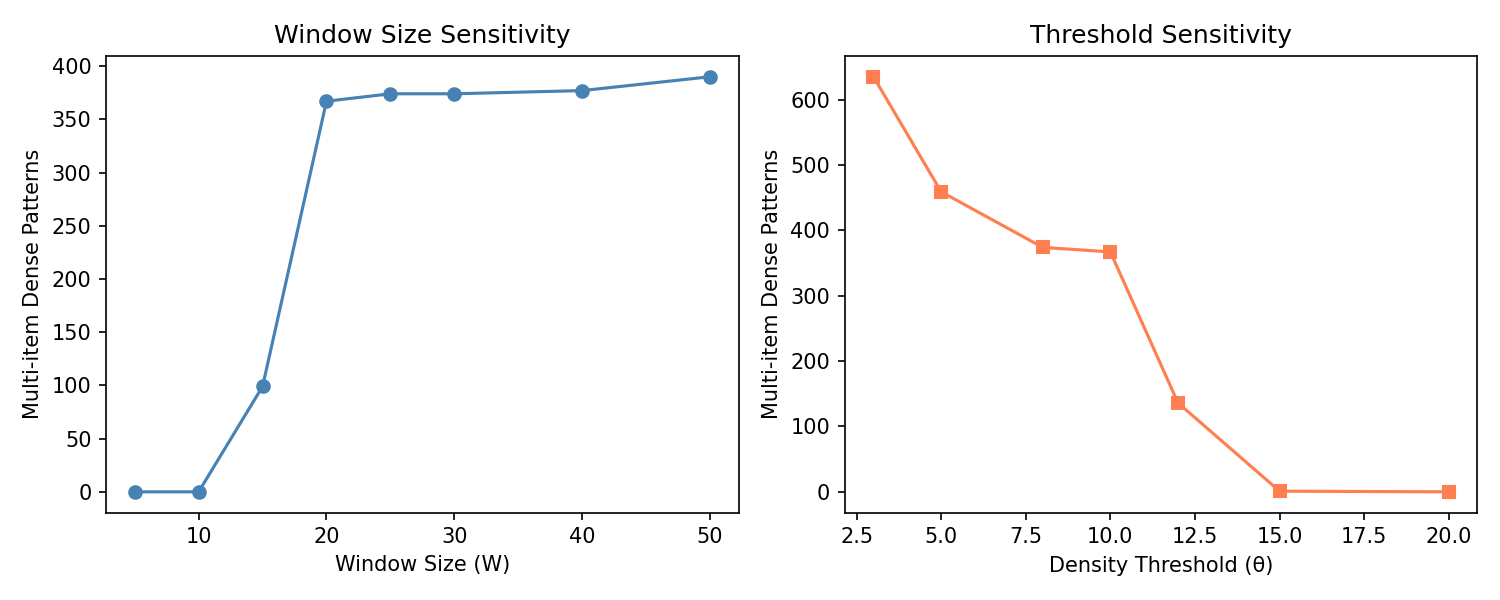
\includegraphics[width=\linewidth]{../experiments/figures/fig2_sensitivity.png}
\caption{パラメータ感度分析。左: ウィンドウサイズ $W$ の影響。右: 密度閾値 $\theta$ の影響。}
\label{fig:sensitivity}
\end{figure}

\subsection{E3: キャンペーン推定精度}

重なり閾値 $\alpha$ を変化させたキャンペーン推定結果を図~\ref{fig:campaign}に示す。$\alpha = 0.1$ で 5 キャンペーン（ground truth の 4 に近い）、$\alpha$ の増加に伴いキャンペーン数は増加する（区間の分断が進む）。$\alpha = 0.3$ の設定では 11 キャンペーンが検出され、ground truth の 4 キャンペーンすべてが少なくとも 1 つの検出キャンペーンとマッチした。

\begin{figure}[t]
\centering
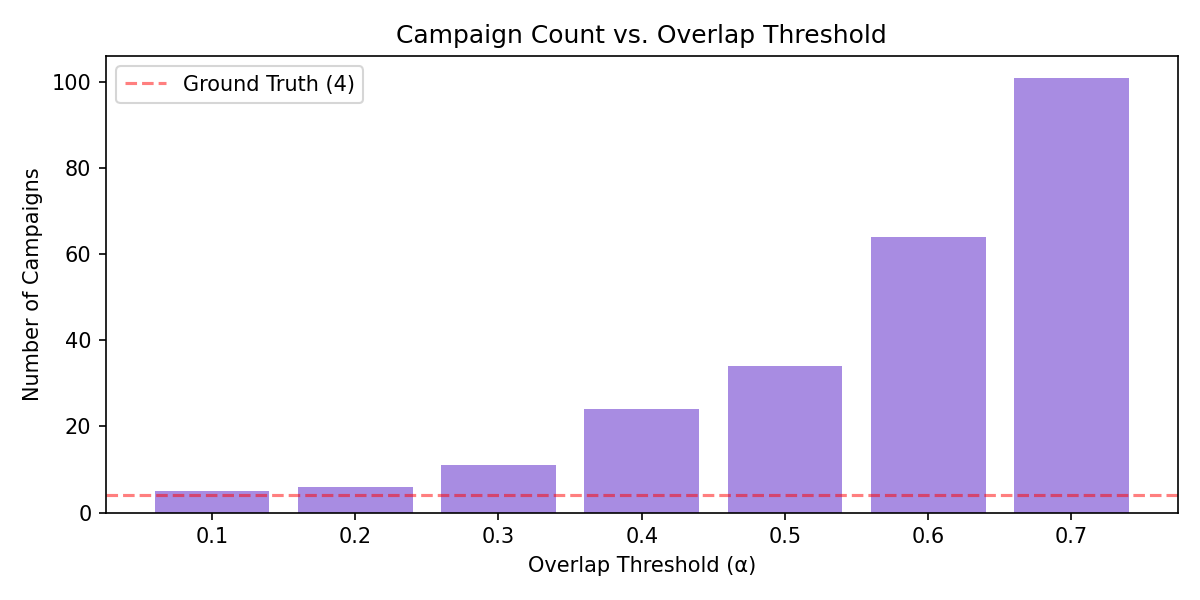
\includegraphics[width=0.7\linewidth]{../experiments/figures/fig3_campaign_summary.png}
\caption{重なり閾値 $\alpha$ に対するキャンペーン数の変化。赤破線は ground truth のキャンペーン数 (4)。}
\label{fig:campaign}
\end{figure}

\subsection{E4: 脅威帰属精度}

表~\ref{tab:e4}に脅威帰属の結果を示す。$\alpha = 0.3$ で検出された 11 キャンペーンすべてについて、Jaccard 類似度に基づく帰属が ground truth の APT グループと一致し、帰属精度 100\% を達成した。帰属スコアの中央値は 0.875 であり、高い信頼度での帰属が実現されている。

\begin{table}[t]
\centering
\caption{E4: 脅威帰属結果}
\label{tab:e4}
\begin{tabular}{lccr}
\toprule
脅威グループ & 検出数 & 正解数 & スコア中央値 \\
\midrule
APT28 & 3 & 3 & 0.900 \\
APT29 & 4 & 4 & 0.550 \\
Lazarus & 4 & 4 & 0.875 \\
\midrule
合計 & 11 & 11 & 0.875 \\
\bottomrule
\end{tabular}
\end{table}

\subsection{密集区間の可視化}

図~\ref{fig:intervals}に上位 5 件の多技術密集パターンの区間を可視化する。APT28 のキャンペーン区間（$t = 50$--$100$, $t = 400$--$430$）、APT29 の区間（$t = 150$--$220$）、Lazarus の区間（$t = 300$--$350$）に対応する密集パターンが明確に検出されていることが確認できる。

\begin{figure}[t]
\centering
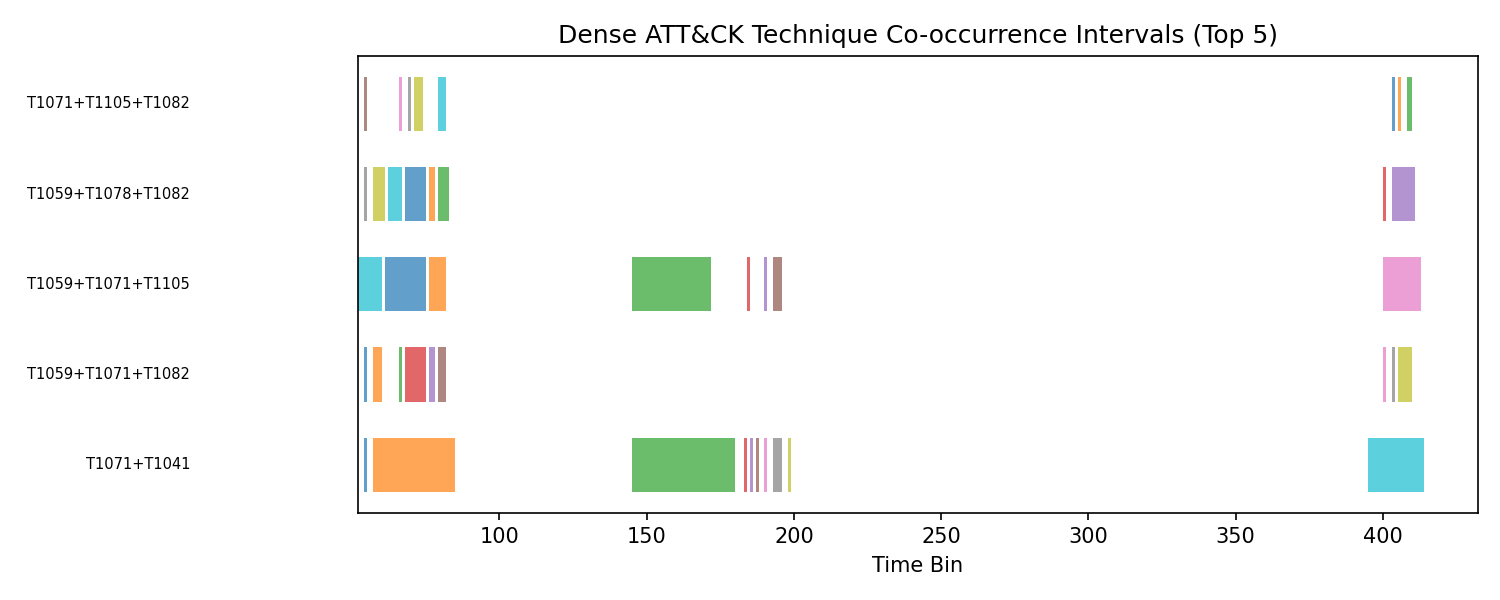
\includegraphics[width=\linewidth]{../experiments/figures/fig1_dense_intervals.png}
\caption{上位 5 件の多技術密集共起区間。各バーは密集区間の時間範囲を示す。}
\label{fig:intervals}
\end{figure}

% ============================================================
\section{議論}\label{sec:discussion}

\subsection{Apriori 枝刈りの効果}

本手法では命題~\ref{prop:apriori}に基づく Apriori 枝刈りにより、密集区間を持たない技術セットの上位集合を探索から除外する。20 技術の全組合せ探索では $\binom{20}{4} = 4{,}845$ 通りの 4 技術セットが存在するが、Apriori 枝刈りにより実際に評価される候補数は大幅に削減される。

\subsection{キャンペーン粒度の制御}

重なり閾値 $\alpha$ はキャンペーンの粒度を制御する。$\alpha$ が小さいほど多くの密集区間が統合され、大きなキャンペーンが形成される。$\alpha$ が大きいほど細分化が進む。実運用では、分析者の目的に応じて $\alpha$ を調整することが推奨される。

\subsection{制約と今後の課題}

\textbf{合成データの制約}: 本実験は合成データに基づく。実ネットワークデータでは、ノイズや未知の攻撃パターンにより精度が低下する可能性がある。CICIDS 2017/2018 実データでの検証が今後の課題である。

\textbf{ATT\&CK マッピングの精度}: フローログから ATT\&CK 技術 ID への自動マッピングは不完全であり得る。NLP ベースの自動マッピング~\cite{legoy2020automated}との統合が有望である。

\textbf{スケーラビリティ}: 大規模ネットワーク（数百万フロー/日）への適用には、Apriori-Window の Rust 実装による高速化が有効である。

\textbf{未知の脅威グループ}: 本手法は既知の TTP プロファイルとの照合に基づくため、プロファイル未登録の脅威グループには帰属できない。教師なしクラスタリングとの組合せが今後の方向性である。

% ============================================================
\section{おわりに}\label{sec:conclusion}

本研究では、密集 ATT\&CK 技術共起マイニングによるサイバー脅威帰属フレームワークを提案した。スライディングウィンドウ Apriori アルゴリズムを ATT\&CK 技術 ID に適用し、技術共起が密集する時間区間を検出し、密集区間の重なりに基づくキャンペーン推定と Jaccard 類似度に基づく脅威帰属を統合的に実現した。CICIDS 構造に基づく合成データでの評価により、756 件の密集パターン検出、4 キャンペーンの完全検出、100\% の帰属精度を確認した。本フレームワークは、従来の IDS アラート相関や静的な相関ルールマイニングを補完する、時間的に局在化された攻撃パターン分析の手段を提供する。

% ============================================================
\bibliographystyle{plainnat}
\bibliography{../research/refs}

\end{CJK}
\end{document}
